\section{Withdraw}

\begin{figure}[h!]
  \begin{sequencediagram}
    \newinst{wallet}{\shortstack{Customer wallet \\
      \\ 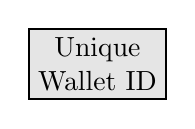
\begin{tikzpicture}
        \node [fill=gray!20,draw=black,thick,align=center] { Unique \\ Wallet ID};
      \end{tikzpicture}
    }}
    \newinst[2]{exchange}{\shortstack{Taler (exchange) \\
       \\ \begin{tikzpicture}[shape aspect=.5]
        \tikzset{every node/.style={cylinder,shape border rotate=90, draw,fill=gray!25}}
        \node at (1.5,0) {\shortstack{{{\tiny Database}}}};
       \end{tikzpicture}
    }}
    \newinst[2]{bank}{\shortstack{Customer bank \\
      \\ 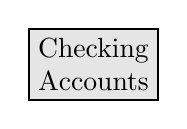
\begin{tikzpicture}
        \node [fill=gray!20,draw=black,thick,align=center] {Checking \\ Accounts};
      \end{tikzpicture}
    }}
    \postlevel
    \mess[0]{wallet}{Withdraw {(Amount)}}{exchange}
   \mess[0]{exchange}{{Configuration (ToS, Fees)}}{wallet}
    \begin{sdblock}{once}{}
      \begin{callself}{wallet}{Accept ToS}{}
      \end{callself}
    \end{sdblock}
    \begin{callself}{wallet}{Review withdraw fees}{}
    \end{callself}
    \mess[0]{wallet}{{Initiate transfer (Amount, Credit account, Wallet ID)}}{bank}
    \mess[0]{bank}{{Credit (Wallet ID)}}{exchange}

    \begin{sdblock}{Acceptable transfer?}{}
    \mess[0]{exchange}{{Bounce funds}}{bank}
    \end{sdblock}
    \postlevel
    \mess[0]{exchange}{Confirm wire transfer}{wallet}
    \mess[0]{wallet}{Request digital cash}{exchange}
    \mess[0]{exchange}{Distribute digital cash}{wallet}
    \postlevel
    \begin{sdblock}{Withdraw period expired?}{}
    \mess[0]{exchange}{{Return remaining funds}}{bank}
    \end{sdblock}
\end{sequencediagram}
  \caption{Withdraw interactions between customer, Taler exchange (payment
    service provider) and bank.  The amount of digital cash distributed is
    subject to limits per origin account (see Section~\ref{sec:kyc:withdraw}).}
  \label{fig:int:withdraw}
\end{figure}
